% Standalone TikZ figure: mAP Calculation Visualization
% For Chapter 7: Reward Function Engineering
\documentclass[tikz,border=10pt]{standalone}
\usepackage{tikz}
\usepackage{amsmath}
\usetikzlibrary{arrows.meta, positioning, shapes.geometric, calc, patterns, decorations.pathreplacing}

\begin{document}
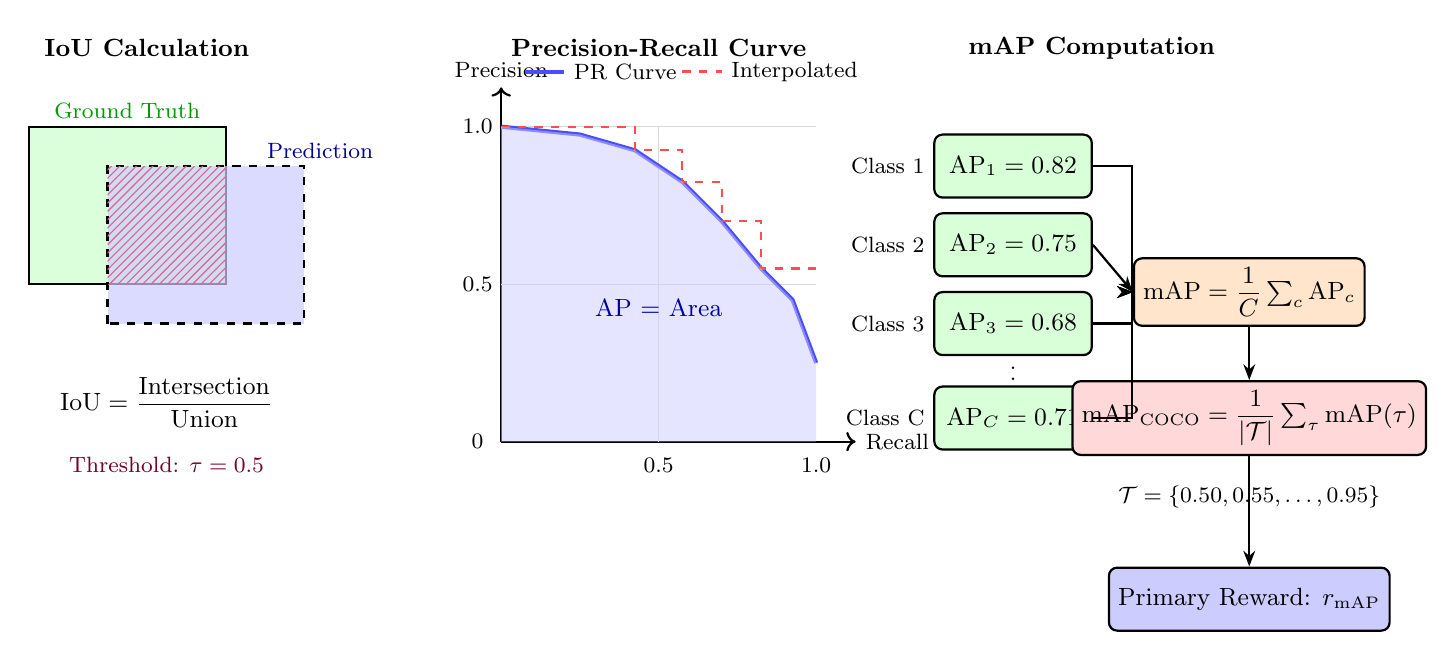
\begin{tikzpicture}[
    node distance=1.2cm and 1.5cm,
    every node/.style={font=\small},
    box/.style={rectangle, draw, thick, minimum width=2cm, minimum height=0.8cm, align=center, rounded corners=3pt},
    arrow/.style={-{Stealth[length=2mm]}, thick},
    label/.style={font=\footnotesize},
    title/.style={font=\bfseries\small}
]

% ============ IoU CALCULATION (LEFT) ============
\node[title] at (0, 3.5) {IoU Calculation};

% Ground truth box
\draw[thick, fill=green!20, fill opacity=0.7] (-1.5, 0.5) rectangle (1, 2.5);
\node[label, green!60!black] at (-0.25, 2.7) {Ground Truth};

% Predicted box
\draw[thick, fill=blue!20, fill opacity=0.7, dashed] (-0.5, 0) rectangle (2, 2);
\node[label, blue!60!black] at (2.2, 2.2) {Prediction};

% Intersection area
\fill[pattern=north east lines, pattern color=purple!60] (-0.5, 0.5) rectangle (1, 2);

% IoU formula
\node[align=center] at (0.25, -1) {$\text{IoU} = \dfrac{\text{Intersection}}{\text{Union}}$};
\node[label, purple!60!black] at (0.25, -1.8) {Threshold: $\tau = 0.5$};

% ============ PRECISION-RECALL CURVE (CENTER) ============
\node[title] at (6.5, 3.5) {Precision-Recall Curve};

% Axes
\draw[thick, ->] (4.5, -1.5) -- (4.5, 3) node[above, label] {Precision};
\draw[thick, ->] (4.5, -1.5) -- (9, -1.5) node[right, label] {Recall};

% Axis labels
\node[label] at (4.2, 2.5) {1.0};
\node[label] at (4.2, 0.5) {0.5};
\node[label] at (4.2, -1.5) {0};
\node[label] at (6.5, -1.8) {0.5};
\node[label] at (8.5, -1.8) {1.0};

% Grid lines
\draw[gray!30] (4.5, 0.5) -- (8.5, 0.5);
\draw[gray!30] (4.5, 2.5) -- (8.5, 2.5);
\draw[gray!30] (6.5, -1.5) -- (6.5, 2.5);

% PR curve (smooth approximation)
\draw[thick, blue!70, line width=1.5pt]
    (4.5, 2.5) -- (5.5, 2.4) -- (6.2, 2.2) -- (6.8, 1.8) -- (7.3, 1.3) -- (7.8, 0.7) -- (8.2, 0.3) -- (8.5, -0.5);

% Interpolated precision (step function)
\draw[thick, red!70, dashed]
    (4.5, 2.5) -- (6.2, 2.5) -- (6.2, 2.2) -- (6.8, 2.2) -- (6.8, 1.8) -- (7.3, 1.8) -- (7.3, 1.3) -- (7.8, 1.3) -- (7.8, 0.7) -- (8.5, 0.7);

% Shaded area under curve (AP)
\fill[blue!20, opacity=0.5]
    (4.5, -1.5) -- (4.5, 2.5) -- (5.5, 2.4) -- (6.2, 2.2) -- (6.8, 1.8) -- (7.3, 1.3) -- (7.8, 0.7) -- (8.2, 0.3) -- (8.5, -0.5) -- (8.5, -1.5) -- cycle;

% Legend
\draw[thick, blue!70, line width=1.5pt] (4.8, 3.2) -- (5.3, 3.2);
\node[label, right] at (5.3, 3.2) {PR Curve};
\draw[thick, red!70, dashed] (6.8, 3.2) -- (7.3, 3.2);
\node[label, right] at (7.3, 3.2) {Interpolated};

% AP annotation
\node[align=center, blue!60!black] at (6.5, 0.2) {AP = Area};

% ============ mAP AGGREGATION (RIGHT) ============
\node[title] at (12, 3.5) {mAP Computation};

% Class AP boxes
\node[box, fill=green!15] (ap1) at (11, 2) {$\text{AP}_1 = 0.82$};
\node[box, fill=green!15] (ap2) at (11, 1) {$\text{AP}_2 = 0.75$};
\node[box, fill=green!15] (ap3) at (11, 0) {$\text{AP}_3 = 0.68$};
\node[label] at (11, -0.6) {$\vdots$};
\node[box, fill=green!15] (apc) at (11, -1.2) {$\text{AP}_C = 0.71$};

% Aggregation
\node[box, fill=orange!20, minimum width=2.5cm] (map) at (14, 0.4) {$\text{mAP} = \dfrac{1}{C}\sum_c \text{AP}_c$};

% IoU threshold averaging
\node[box, fill=red!15, minimum width=3cm] (coco) at (14, -1.2) {$\text{mAP}_{\text{COCO}} = \dfrac{1}{|\mathcal{T}|}\sum_{\tau} \text{mAP}(\tau)$};

% Threshold list
\node[label, align=center] at (14, -2.2) {$\mathcal{T} = \{0.50, 0.55, \ldots, 0.95\}$};

% Arrows
\draw[arrow] (ap1.east) -- ++(0.5,0) |- (map.west);
\draw[arrow] (ap2.east) -- (map.west);
\draw[arrow] (ap3.east) -- ++(0.5,0) |- (map.west);
\draw[arrow] (apc.east) -- ++(0.5,0) |- (map.west);
\draw[arrow] (map.south) -- (coco.north);

% Class labels
\node[label, left] at (10, 2) {Class 1};
\node[label, left] at (10, 1) {Class 2};
\node[label, left] at (10, 0) {Class 3};
\node[label, left] at (10, -1.2) {Class C};

% Final result
\node[box, fill=blue!20, thick] (result) at (14, -3.5) {Primary Reward: $r_{\text{mAP}}$};
\draw[arrow] (coco.south) -- (result.north);

\end{tikzpicture}
\end{document}
